% !TEX program = latexmk
%% AINA-2027 submission (Springer Lecture Notes, class svproc; max. 12 pages incl. references).
\documentclass{svproc}

\usepackage{url}
\def\UrlFont{\rmfamily}
\usepackage{graphicx}
\usepackage{booktabs}
\usepackage{array}
\usepackage{amsmath,amssymb}
\usepackage{algorithm}
\usepackage{algpseudocode}
\usepackage{tikz}
\usepackage{xcolor}
\usepackage{listings}
\lstdefinelanguage{SPARQL}{morekeywords={SELECT,WHERE,VALUES,BIND,IF,AS,ORDER,BY,DESC,OPTIONAL,PREFIX,INSERT,COUNT,SUM,GROUP},sensitive=true,morestring=[b]",morecomment=[l]{\#}}
\lstset{language=SPARQL,basicstyle=\scriptsize\ttfamily,keywordstyle=\bfseries\color{blue!55!black},stringstyle=\color{orange!60!black},commentstyle=\itshape\color{gray},frame=tb,framerule=0.4pt,backgroundcolor=\color{gray!6},numbers=left,numberstyle=\tiny\color{gray},numbersep=4pt,xleftmargin=1.2em,aboveskip=4pt,belowskip=2pt,columns=fullflexible,keepspaces=true,captionpos=t}
\renewcommand{\lstlistingname}{Listing}
\AtBeginDocument{\renewcommand{\thelstlisting}{\arabic{lstlisting}}}
\usetikzlibrary{positioning,arrows.meta,shapes.geometric,fit,backgrounds,calc}

\emergencystretch=1.5em
\newcommand{\pending}[1]{\textcolor{red}{\textbf{[PENDING: #1]}}}
\begin{document}
\mainmatter

\title{Contextual Assistance for Users of Ridesharing Services: Explainable Offer Ranking with an OWL Context Model}
\titlerunning{Contextual Assistance for Ridesharing}

%% Review mode: set \anontrue for a double-blind (anonymous) PDF.
\newif\ifanon
\anonfalse
\ifanon
\author{Anonymous Author(s)}
\authorrunning{Anonymous et al.}
\tocauthor{Anonymous Author(s)}
\institute{Affiliation removed for review}
\else
\author{Elisa de F\'atima Andrade Soares \and Breno Jos\'e Ribeiro de Vasconcelos \and
Carlos Andr\'e Guimar\~aes Ferraz}
\authorrunning{E. F. A. Soares et al.}
\tocauthor{Elisa de F\'atima Andrade Soares, Breno Jos\'e Ribeiro de Vasconcelos, Carlos Andr\'e Guimar\~aes Ferraz}
\institute{Centro de Inform\'atica (CIn), Universidade Federal de Pernambuco (UFPE), Recife, Brazil\\
\email{\textrm{\{}efas, bjrv, cagf\textrm{\}}@cin.ufpe.br}}
\fi

\maketitle

\begin{abstract}
Carpool rankings are opaque and cannot be checked. We present ContexCarpool, a context-aware architecture whose ranking rules, rationale queries and provenance are expressed in W3C standards (OWL, SHACL, SPARQL 1.1 Update, PROV-O), so that any compliant engine, including one in the passenger's mobile browser, can re-execute them. Given authentic listings, the phone recomputes a published ranking and each rationale to check them; it adds remarks from its position and clock without sending them; it groups offers by whether they can be reached on foot or only by car and orders each group by total cost; and after the trip it computes the fare from the distances recorded by both parties, so an early drop-off is paid pro rata. Position, clock, trip records and prices are simulated or modeled. On synthetic listings and on real departure points and times from the French carpool registry, three engines (Jena, rdflib, Oxigraph) pass conformance tests against a separate Python implementation. The order is stable under weight perturbation (Kendall $\tau = 0.88$), but 10--20\% price noise changes the top of the list. On an iPhone and an Android phone over 4G and 5G, ranking 100 offers takes 24--26\,ms on the phone after the offers are downloaded, while the engine's first load takes 1.2--3.1\,s.
\keywords{mobile and context-aware computing, Semantic Web, SPARQL, recomputable ranking, ridesharing}
\end{abstract}

\section{Introduction}\label{sec:intro}
In \emph{peer carpooling}, a private driver offers spare seats on a trip already planned~\cite{si2023}. A passenger compares many similar offers on price, comfort and booking friction (instant booking or driver approval), but research has mostly optimized system-level objectives such as matching and detour~\cite{agatz2012}, and recent recommenders rank options~\cite{Psaraftis2024QERide} without explaining the order. EU law requires marketplaces to disclose their main ranking parameters~\cite{eudsa2022}, but only in aggregate. The question \emph{why is this offer above that one?} is rarely answered in a form that anyone can check.

We address a design problem: \emph{how can carpool offers be ranked so that a third party, including the passenger's own phone, can check each per-offer rationale and the fare actually charged, with off-the-shelf tools and only parameters a platform would disclose anyway, at interactive cost?} Context has three levels here: the \emph{search} (the competing offers determine each offer's relative cost), the \emph{device} (position and clock, simulated in the prototype) and the \emph{trip} (where the passenger actually got off). In ContexCarpool, a SHACL~\cite{w3cshacl2017} contract validates listings, an OWL~\cite{w3cowl2} model represents them in RDF, rules written as SPARQL~\cite{w3csparql2013} 1.1 Update~\cite{w3cupdate2013} operations infer facts and record each firing with PROV-O~\cite{w3cprov2013}, and SPARQL queries rank the offers and build each rationale. The weights are a documented prior, not fitted to preference data. Each research question has a result that would refute it:
\begin{itemize}
  \item[\textbf{RQ1}] Does each criterion carry information that the others do not? \emph{Refuted if} one is predictable from the other two (cross-validated $R^2 \ge 0.9$).
  \item[\textbf{RQ2}] Is the ranking robust to the weight prior and to data changes? \emph{Refuted if} the mean Kendall $\tau_b$ ($\tau$ below) falls below $0.7$ or the mean top-$k$ overlap ($k = 3$ for 20-offer pages, 10 otherwise) below $80\%$, under $\pm 0.1$ weight perturbations or 5--20\% perturbations of the offers' attributes.
  \item[\textbf{RQ3}] Is the standards-based pipeline cheap enough on a server? \emph{Refuted if} a result page takes over 0.1\,s, the limit for an instantaneous response~\cite{nielsen1993}.
  \item[\textbf{RQ4}] Can the passenger's phone run it? \emph{Refuted if} ranking a 100-offer search (excluding loading) takes over 0.1\,s on the tested phones.
\end{itemize}
\textbf{Contributions.} (i) a context-aware architecture whose public order uses only public data, so it can be audited, while device and trip context act on the phone; (ii) an OWL ontology aligned with schema.org and PROV-O, a SHACL contract, fifteen SPARQL Update rules and eight competency questions; (iii) conformance across three engines, in the browser and by an auditor, under a stated threat model; (iv) a mobile client that checks the published ranking, gives a personal view by total access cost and demonstrates, with simulated distance records, a fare recomputed after the trip; and (v) a reproducible benchmark\footnote{Code, ontology, rules, queries and data: \url{https://github.com/elisandrade21/contexcarpool}.} with real registry data and two phones. A companion paper shares the score logic and base generator; all results here are new.

\section{Related Work}\label{sec:related}
\begin{table}[t]
  \caption{Closest work: carpool or ridesharing; semantic (OWL/RDF/rules); explains each item; runs on the user's device; output recomputable or checkable by a third party ($\checkmark$ addressed, -- not addressed or not reported).}
  \label{tab:rw}
  \centering\scriptsize
  \begin{tabular}{@{}llccccc@{}}
    \toprule
    Work & Venue & Carpool & Semantic & Explains & On device & Checkable \\
    \midrule
    Hsieh~\cite{Hsieh2017CarPooling} & AINA'17 & $\checkmark$ & -- & -- & -- & -- \\
    Liu and Li~\cite{Liu2021SemanticTrajectory} & AINA'21 & $\checkmark$ & -- & -- & -- & -- \\
    Jenevain et al.~\cite{Jenevain2024ContextOntology} & AINA'24 & -- & $\checkmark$ & -- & -- & -- \\
    QE-Ride~\cite{Psaraftis2024QERide} & IEEE Access'24 & $\checkmark$ & -- & -- & -- & -- \\
    RideMATCHain~\cite{Gramegna2023RideMATCHain} & ICWE-W'22 & $\checkmark$ & $\checkmark$ & $\checkmark$ & -- & -- \\
    B-Ride~\cite{Baza2021BRide} & TNSE'21 & $\checkmark$ & -- & -- & $\checkmark$ & $\checkmark$ \\
    Kalidas et al.~\cite{Kalidas2026ELSA} & TORS'26 & -- & $\checkmark$ & $\checkmark$ & -- & -- \\
    Lee et al.~\cite{Lee2020ContextRec} & ISWC'20 & -- & $\checkmark$ & $\checkmark$ & $\checkmark$ & -- \\
    Samsung PDE~\cite{Crocker2025Pocket} & ISWC'25 & -- & $\checkmark$ & -- & $\checkmark$ & -- \\
    Tiny-ME Wasm~\cite{Loseto2024TinyME} & ICWE-W'23 & -- & $\checkmark$ & -- & $\checkmark$ & -- \\
    HyLAR~\cite{Terdjimi2015HyLAR} & ESWC-W'15 & -- & $\checkmark$ & -- & $\checkmark$ & -- \\
    Leiden Ranking OE~\cite{vanEck2024Leiden} & Blog'24 & -- & -- & -- & -- & $\checkmark$ \\
    zkRDF~\cite{Braun2026ZkSparql} & ESWC'26 & -- & $\checkmark$ & -- & -- & $\checkmark$ \\
    \midrule
    \textbf{ContexCarpool} &  & $\checkmark$ & $\checkmark$ & $\checkmark$ & $\checkmark$ & $\checkmark$ \\
    \bottomrule
  \end{tabular}
\end{table}

Table~\ref{tab:rw} compares the closest work. In a title screening of AINA 2017--2026 (2,406 papers with workshops, abstracts read for about 120 candidates; list in the repository), only three relate to carpooling, all platform-side: trajectory matching~\cite{Hsieh2017CarPooling}, demand mining~\cite{Liu2021SemanticTrajectory} and Mobility as a Service~\cite{Falanga2024MaaS}; AINA work on semantic context uses rules~\cite{Amato2017VisitingPath} and context modules~\cite{Amara2024ContextForecast,Jenevain2024ContextOntology}. Ridology~\cite{wagih2020} models ridesharing trips, not the offer a passenger ranks. For provenance we use PROV-O, and for rules SPARQL Update rather than SWRL, SHACL-AF or RIF~\cite{w3crif2013}, which none of our engines executes. Ranking labels describe a ranking's weights and stability~\cite{Yang2018RankingFacts}; open rankings can be recomputed by third parties~\cite{vanEck2024Leiden}; open indexes let users rank locally~\cite{Hendriksen2026OpenIndex}; zero-knowledge proofs certify SPARQL results while hiding data~\cite{Braun2026ZkSparql}; audits check systems against documentation~\cite{raji2020}. On-device RDF recommendation runs on phones~\cite{Lee2020ContextRec,Crocker2025Pocket} and description logics in the browser~\cite{Loseto2024TinyME}. Unlike third-party recomputation of open rankings, we let the passenger's own device re-execute a ranking that a server published and check each item's score, position and rationale; compared with publishing a hashed script, standard rules can be re-executed by independent engines and carry provenance that a third party can query; we also apply the same rule mechanism to the fare after the trip, which B-Ride settles on a blockchain~\cite{Baza2021BRide}.

\section{ContexCarpool}\label{sec:arch}
\subsection{Architecture and Context Model}
Four layers connect platforms to passengers: platforms expose JSON listings; preprocessing maps them to SHACL-valid RDF; contextual assistance ranks the listings of one search and explains each rank; front-ends show them. Contextual assistance runs as a stateless service (\texttt{POST /rank}, Jena) or in the browser.



\textsf{Travel}, \textsf{Car}, \textsf{Place} and \textsf{Participant} specialize the schema.org classes Trip, Car, Place and Person, and patterns follow Ridology~\cite{wagih2020}; the module we add covers derived offer properties, comfort levels, trade-offs, the device context, trip records and remarks. Each rule is a \textsf{prov:Plan}; each firing is a \textsf{prov:Activity} qualified by the reasoner and the rule; each inferred fact is a \textsf{prov:Entity} generated by the firing and derived from its inputs (a fact is tied to its triple only through \textsf{rdf:value}; RDF 1.2 triple terms could close this gap). Functional properties, disjoint classes and pairwise distinct levels make conflicting inferences inconsistent. Eight competency questions (CQ1--CQ8) determined the new terms; the ontology has 14 classes, 22 properties, 30 named individuals and 9 alignments (4 to schema.org, 5 to PROV-O).

\subsection{Score, Rules and Explanation}\label{sec:rules}
With $d$ free seats, rules R1--R4 infer \textsf{VeryComfortable} ($d \ge 4$), \textsf{Comfortable} ($d = 3$), \textsf{Bearable} ($d = 2$) or \textsf{Uncomfortable} ($d \le 1$), giving $f_C = 10, 7.5, 5, 2.5$ (15.2, 34.9, 32.2, 17.7\% of offers). Cost $f_K \in [0,10]$ is the reversed percentile of the price per km within the search, so cost ranks offers within one market but does not compare markets. Booking gives $f_B = 10$ (automatic) or 2.5 (driver approval). The score is $S = 0.4 f_C + 0.4 f_K + 0.2 f_B$: rank-sum surrogate weights~\cite{barron1996} of the ordering comfort = cost $>$ booking reported by willingness-to-share studies~\cite{si2023}, rounded; a prior, since those studies concern sharing a ride, not choosing among offers. Rules R5--R8 infer a trade-off for the cheapest or most expensive quarter of the search with automatic or manual booking (e.g., cheap \emph{but} needs approval) and change only the rationale. Each rule is one SPARQL 1.1 Update \texttt{INSERT\,\dots\,WHERE} that asserts the fact and its PROV-O record, with node IRIs derived from the offer so that every engine builds the same graph; rules are non-recursive and run once, after the cost percentiles are computed. One query (CQ1) computes $S$, orders the offers and builds each rationale from asserted and inferred triples; since $S$ is additive, CQ5 answers ``why is A above B?'' exactly (FR-0271 outranks FR-0057 by 1.62 points: 1.50 from booking, 0.12 from cost). Fig.~\ref{fig:pipeline} follows one offer through the trace.

\begin{figure}[t]
  \centering
  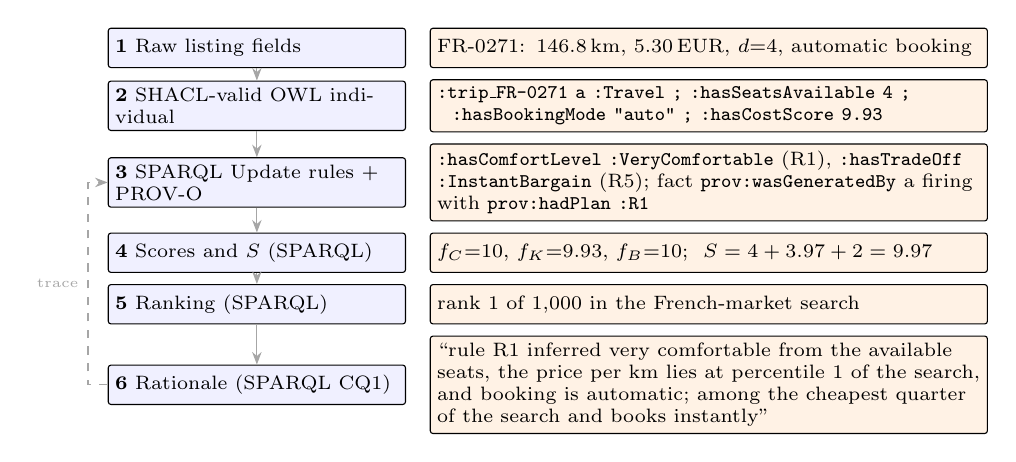
\begin{tikzpicture}[
    box/.style={draw, rounded corners=1pt, fill=blue!6, font=\scriptsize, inner sep=2.5pt, align=left, text width=3.6cm, minimum height=0.5cm},
    ex/.style={draw, rounded corners=1pt, fill=orange!10, font=\scriptsize, inner sep=2.5pt, align=left, text width=6.9cm, minimum height=0.5cm},
    arr/.style={-{Stealth[length=1.6mm]}, gray!70},
    node distance=0.14cm]
    \node[ex] (e1) {FR-0271: 146.8\,km, 5.30\,EUR, $d{=}4$, automatic booking};
    \node[ex, below=of e1] (e2) {\texttt{:trip\_FR-0271 a :Travel ; :hasSeatsAvailable 4 ;}\\\texttt{\ \ :hasBookingMode "auto" ; :hasCostScore 9.93}};
    \node[ex, below=of e2] (e3) {\texttt{:hasComfortLevel :VeryComfortable} (R1), \texttt{:hasTradeOff :InstantBargain} (R5); fact \texttt{prov:wasGeneratedBy} a firing with \texttt{prov:hadPlan :R1}};
    \node[ex, below=of e3] (e4) {$f_C{=}10$, $f_K{=}9.93$, $f_B{=}10$; \ $S = 4 + 3.97 + 2 = 9.97$};
    \node[ex, below=of e4] (e5) {rank 1 of 1{,}000 in the French-market search};
    \node[ex, below=of e5] (e6) {``rule R1 inferred very comfortable from the available seats, the price per km lies at percentile 1 of the search, and booking is automatic; among the cheapest quarter of the search and books instantly''};
    \node[box, left=0.3cm of e1] (raw) {\textbf{1} Raw listing fields};
    \node[box, left=0.3cm of e2] (proj) {\textbf{2} SHACL-valid OWL individual};
    \node[box, left=0.3cm of e3] (rule) {\textbf{3} SPARQL Update rules + PROV-O};
    \node[box, left=0.3cm of e4] (score) {\textbf{4} Scores and $S$ (SPARQL)};
    \node[box, left=0.3cm of e5] (rank) {\textbf{5} Ranking (SPARQL)};
    \node[box, left=0.3cm of e6] (expl) {\textbf{6} Rationale (SPARQL CQ1)};
    \foreach \a/\b in {raw/proj,proj/rule,rule/score,score/rank,rank/expl} \draw[arr] (\a) -- (\b);
    \draw[arr, dashed] (expl.west) -- ++(-0.25,0) |- (rule.west) node[pos=0.25, left, font=\tiny] {trace};
  \end{tikzpicture}
  \caption{Explanation trace of the top offer of a French search (percentile 1 = cheapest 1\%).}
  \label{fig:pipeline}
\end{figure}

\subsection{Device Context, Personal View and Fare}\label{sec:mobile}
\textbf{Device context.} The phone asserts its position and clock as a \textsf{DeviceContext} (simulated by buttons in the prototype; a deployment would read the GPS), and rules R9--R13 combine them with each offer's pickup and departure: pickup within 800\,m (R9) or beyond 5\,km (R10); leaves within the hour (R11); not reachable on foot at 5\,km/h before departure (R12); beyond 5\,km or too late on foot but reachable by car at 25\,km/h (R13). Thresholds are illustrative; SPARQL has no trigonometry, so the device asserts the cosine of its latitude. These remarks never change the public order, which must not depend on private data.

\textbf{Personal view.} On the phone only, CQ7 groups the offers, in this order, into those reachable on foot, those reachable only by car (R13) and those not reachable in time; within each group the app orders offers (in JavaScript, not by the rules) by total cost, the carpool price plus a ride-hailing fare the passenger enters for the car group, so an offer whose pickup needs a taxi moves below those within walking distance.

\textbf{Fare after the trip.} Each phone records the distance the passenger actually traveled as a \textsf{TripRecord}; both phones exchange the two records and run R14--R15. If the records agree within 5\% of the trip, the fare is the agreed price per km times the mean recorded distance, capped at the booked distance (R14); otherwise the trip is flagged as disputed (R15). The client runs R14--R15 and CQ8 in the browser, so both phones compute the same fare from the same public rule, and an early drop-off is paid pro rata. In the prototype both records are entered on one phone; reading them from GPS and exchanging them between phones are future work, and a disputed trip goes to the platform's usual support. The rule needs distance errors of about 2\% or less: with simulated records, honest trips are disputed in 2.3\% of cases at 2\% error but in 34\% at 5\% (Sect.~\ref{sec:verif}), so we present it as a demonstration, not a validated mechanism. Each party can shift the fare by at most half the tolerance without being flagged. Unlike B-Ride, which pays the distance traveled through a blockchain and continuous payment~\cite{Baza2021BRide}, the fare is agreed before the trip and reduced by a public rule fixed in advance.

\textbf{Checking the published ranking.} The phone recomputes $S$, the order and each rationale from public offer data only and compares them with what the server published; private remarks stay out of the comparison. The client code must come from a source independent of the server (e.g., an app store or the auditor), or the check is circular; our prototype serves it from the server under test. A match shows that the output follows the public rules and data, not that the data are true or that every user saw the same ranking. The client is a web page running Oxigraph compiled to WebAssembly with the same files (Fig.~\ref{fig:app}); SHACL is not checked on the phone (Oxigraph has no SHACL engine), and the server computes $f_K$ by sorting, with the same values. The exact position and clock are not sent for the check (the speed test sends them, to time the server with the same rules), but the searched market is, and downloading offers reveals the IP address. Offers expose drivers' departure points and times. \textbf{Threat model.} We assume authentic listings and trip records and honest but noisy phones; the check detects outputs that deviate from the public rules, not forged inputs, spoofed GPS, collusion or per-user rankings, which would need signed listings in an append-only log.

\begin{figure}[t]
  \centering
  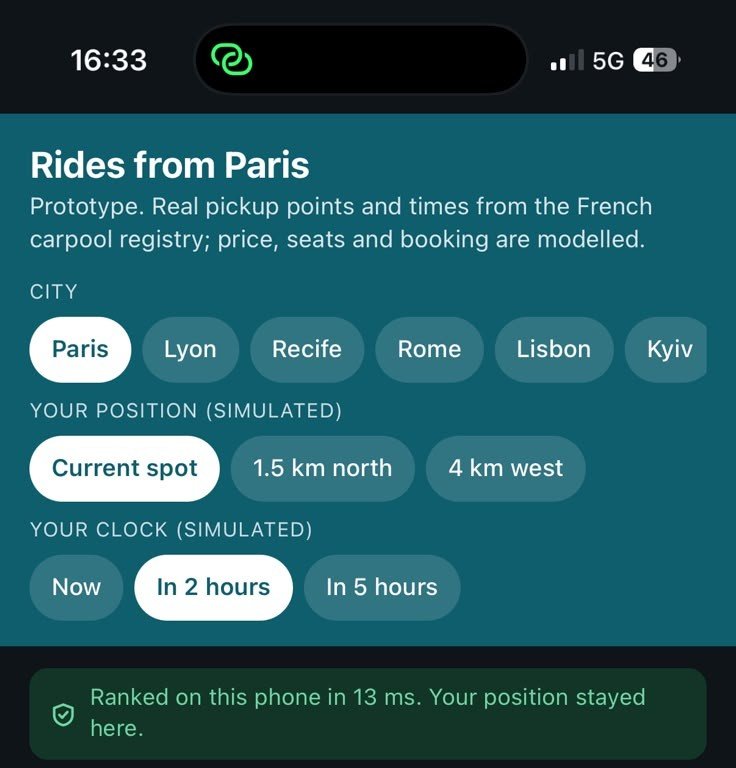
\includegraphics[height=2.6cm]{figs/app_iphone.jpg}\hspace{2mm}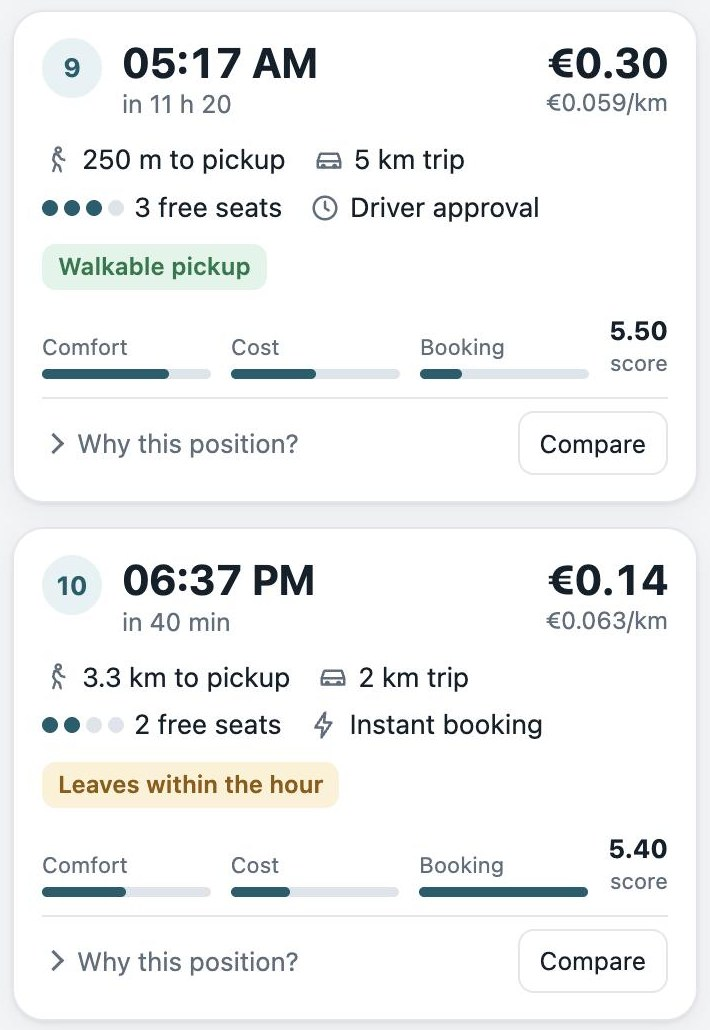
\includegraphics[height=2.6cm]{figs/app_offer.jpg}\hspace{2mm}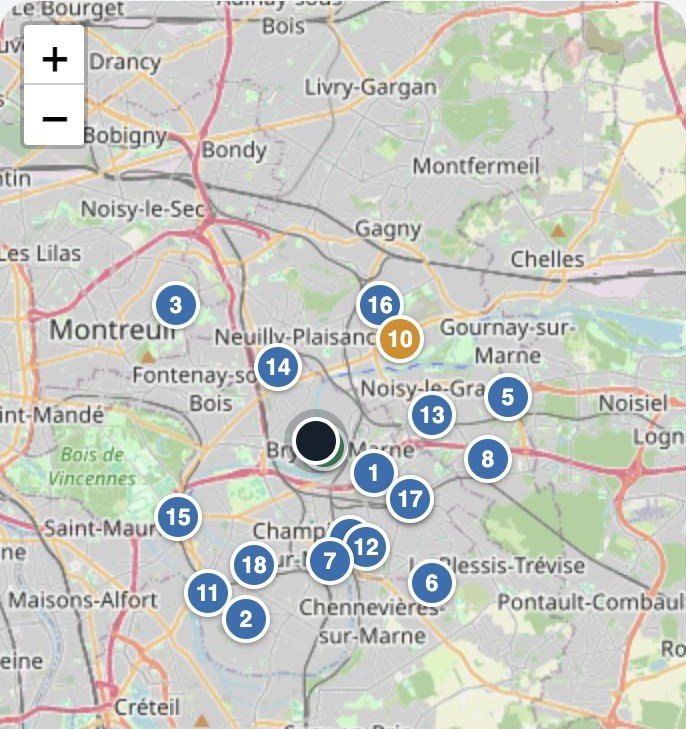
\includegraphics[height=2.6cm]{figs/app_map.jpg}
  \caption{Mobile client (Paris; real pickups and times, modeled prices) on an iPhone over 5G (left) and in a phone-sized browser: two offers with remarks from R9 and R11, and pickups colored by remark.}
  \label{fig:app}
\end{figure}

\section{Evaluation}\label{sec:exp}
\textbf{Setup.} Open listings with the needed fields do not exist, so a seeded generator produces 5,000 listings in five markets with illustrative parameters, and a France scenario (5,000 listings) is calibrated from published BlaBlaCar statistics~\cite{farajallah2019,lambin2026,Blayac2026ShareRide}. Searches are whole markets ($N{=}1{,}000$) or pages of 20 or 100 offers. To exercise the context rules, 60 searches of 100 offers around Recife, Paris, Rome, Lisbon and Kyiv are given illustrative pickups (drawn with a median of 2.5\,km) and departures (5\,min--12\,h), and 30 searches use completed trips from the French carpool registry~\cite{rpc2026} (Paris and Lyon, October 2026): each matches a real passenger trip, with the passenger at its real origin and 20 offers that start and end within 5\,km of its origin and destination and leave within 12\,h, with real departure points, times and distances, with modeled prices, seats and booking modes (so absolute prices are not meaningful). For 30\% of the offers (1,977 simulated trips) the passenger gets off after 50--100\% of the trip; both phones record the distance with 1\% noise, and in 5\% of those trips (122) the driver's phone records the full trip. A Python reference, Jena 4.10, rdflib 7.6 and Oxigraph 0.5.13 run on an Apple M3 Pro laptop; the README regenerates every number except the phone runs.

\subsection{Verification}\label{sec:verif}
\begin{table}[t]
  \caption{Conformance tests (0 differences: identical to the reference, scores within $10^{-9}$).}
  \label{tab:verif}
  \centering\scriptsize
  \begin{tabular}{@{}>{\raggedright}p{3.0cm}>{\raggedright}p{2.6cm}>{\raggedright\arraybackslash}p{6.1cm}@{}}
    \toprule
    Check & Engine & Result \\
    \midrule
    Rules R1--R8, ranking & Jena; rdflib & 5,000 offers (97,500 triples); 30 searches: 0 differences \\
    Consistency, input contract & Jena OWL Mini; Jena SHACL & 2/2 planted contradictions detected; 250/250 defective offers rejected \\
    Tamper detection & rdflib auditor & 6 kinds $\times$ 200: 1,200/1,200 detected, 0/200 false alarms \\
    R1--R13, CQ6 & Oxigraph, rdflib, Jena & 90 searches (6,600 offers): 0 differences; no public order changed \\
    Personal view CQ7 & Oxigraph, rdflib, Jena & 90 searches: 0 differences \\
    Fare R14--R15, CQ8 & Oxigraph, rdflib, Jena & 1,977 trips (113 of 122 overclaims flagged): 0 differences \\
    \bottomrule
  \end{tabular}
\end{table}

Table~\ref{tab:verif} lists conformance tests: they show that engines and rationales are faithful to the model, not that the model is valid for users. The auditor holds only raw fields, assumed authentic, and the public files; an exact recomputation detects any deviation of published scores, order or rationales from the public rules, so tamper detection shows that the audit tool works; it cannot detect false inputs or per-user rankings. Porting to Oxigraph exposed two issues the other engines hide: it rejects a prologue repeated after each update, and its \texttt{xsd:decimal} products overflowed, so a rule silently failed to fire; we declare the prologue once and use \texttt{xsd:double}. In the matched registry searches, R9 fires for 15\% of offers, R11 for 29\%, R12 for 10.5\% and R13 for 9.8\% (no pickup lies beyond 5\,km), and the personal view moves 10.5\% of the offers below those reachable (21\% over all searches). In the simulated trips, the rule flagged 113 of the 122 planted overclaims (in the 9 missed trips the passenger got off after 95\% of the trip, within the tolerance) and no honest trip. With the rule's reference logic on 10,000 honest and 10,000 overclaimed trips per setting, false disputes depend on the relative GPS error, not on trip length (13.8 or 300\,km): at a 5\% tolerance they are 1 in 10,000 at 1\% error, 2.3\% at 2\% and 34\% at 5\% (0.2\% and 19\% if the two phones' errors correlate at 0.5). The 90\% detection of full-trip overclaims follows from drop-offs drawn over 50--100\% of the trip; overclaims within the tolerance go unseen. Server (Jena, sorted percentile) and phone engine (Oxigraph) also produced the same rationale text for all 6,600 offers, after a .5 tie in the cited percentile, rounded differently in double and decimal arithmetic, had made 42 of 9,000 differ in an earlier run.

\subsection{RQ1 and RQ2: Criteria and Robustness}\label{sec:rq2}
RQ1 checks the detector more than the market: in a counterexample where booking is fully determined by comfort, single-criterion correlation ($\rho \approx 0.81$) and ablation ($\tau = 0.86$) miss the redundancy, whereas a cross-validated gradient-boosted model predicting each criterion from the other two finds it ($R^2 = 1.0$). On our data $R^2 \le 0.002$ (up to 0.72 when seats and price are coupled by a Gaussian copula with $\rho = \pm 0.9$), so RQ1 is not refuted, but independence holds by design. As baselines, ordering by price alone or by price per km agrees little with $S$ ($\tau = 0.26$ and $0.51$; top-10 overlap 6\% and 14\%). Perturbing each weight by $\pm 0.1$ gives a mean $\tau = 0.88$ (bootstrap 95\% CI [0.879, 0.880] over 1,000 pages of 100 offers) and top-$k$ overlaps of 87--98.5\%; other weighting methods give similar orders (mean $\tau$: rank-order centroid 0.89, CRITIC 0.78, entropy 0.74). Price noise of 5\% or flipping 5--10\% of booking modes keeps $\tau \ge 0.90$ on synthetic data (0.87--0.89 on the calibrated scenario), but 10--20\% price noise changes the top (top-10 overlap 78\%/60\% on markets, 83\%/70\% on pages, 68--76\% with all perturbations combined): RQ2 is refuted for the top of the list; the overall order keeps $\tau \ge 0.72$, except on calibrated pages at 20\% ($\tau = 0.65$), where RQ2 fails on $\tau$ too.

\subsection{RQ3 and RQ4: Server and Phone}\label{sec:rq4}
\textbf{Server.} Across three stored runs on a laptop, the median time of the pipeline in Jena is 4.2--5.5, 20--21.5\,ms and 1.48--1.51\,s for 20, 100 and 1,000 offers (95th percentile, p95, $\le$ 8.4\,ms, 30\,ms, 1.71\,s), and 2.7--3.2, 5.7--6.0 and 44--49\,ms when the pairwise SPARQL percentile is replaced by sorting; the HTTP service, which sorts the percentile, answers a 100-offer search in 6.7--8.1\,ms (median, one client) and sustains 429--497 requests/s with eight clients. RQ3 is not refuted; a whole 1,000-offer market, which is not a result page, exceeds the limit (1.5\,s) unless the percentile is sorted (44--49\,ms).
\textbf{Phone.} On an iPhone (Safari 26) and an Android phone (Chrome 156), in one session per phone, run once over 4G and once over 5G (one page load per phone; network chosen by hand; an earlier build of the same client), five 100-offer and five 20-offer searches, each repeated 8 times, were ranked on the phone (rules and queries, excluding loading) in 24--26 and 10--15\,ms (median; p95 $\le 33$\,ms): RQ4 is not refuted on these phones. The same searches sent to our server, a free-tier VM in South Carolina (round trip 176--240\,ms), took 268--421 and 226--272\,ms (p95 up to 920\,ms), so the phone answers in less than one round trip; phone and server agreed on score and remark count in all 320 runs. The first load transferred 1.6\,MB for the engine, which started in 1.2\,s (iPhone) and 3.1\,s (Android). Per 100-offer search, the offers and the server's answer are each about 2.4\,kB compressed, so the phone saves no traffic; what it gains is privacy and the ability to check the ranking. Two phones in one session each are a small sample; the server is far from the phones.

\section{Discussion and Conclusion}\label{sec:disc}
\textbf{Why semantic web standards?} For R1--R4 alone, an SQL \texttt{CASE WHEN} expression gives the same ranking; the standards add an input contract, qualified provenance, conflict detection and rules that any compliant engine, including a phone's, can re-execute, which is what makes the public ranking and the fare recomputable by both parties. \textbf{Adoption.} Regulators can require the rules under the DSA~\cite{eudsa2022}; a public registry can host them. \textbf{Threats.} $S$ is a proxy with illustrative weights and thresholds; driver rating and schedule also matter~\cite{si2023}; cost is search-relative and mixes trip lengths; the data are mostly synthetic, and the fare records are simulated. Rationales are faithful to the model, not proof that it reflects what users value~\cite{zhangchen2020}.

We presented ContexCarpool, which ranks carpool offers with rationales that a server, an auditor or the passenger's phone can re-execute, and which uses the same rules to settle the fare after the trip. Next, we will read real GPS traces, fit the weights to preference data, test with users and more phones, and address security: signed listings and trip records, spoofed context and the integrity of the delivered code.

\bibliographystyle{spmpsci}
\bibliography{refs}

\end{document}
